%============================================================
%  MODERN B.SC / M.SC COMPUTER SCIENCE PROJECT REPORT TEMPLATE
%============================================================

\documentclass[12pt,a4paper,oneside]{report}

%------------------------------------------------------------
% PACKAGES
%------------------------------------------------------------
\usepackage[top=20mm, bottom=20mm, left=30mm, right=25mm, headheight=15pt]{geometry}
\usepackage{setspace}            % line spacing
\usepackage{lmodern}             % Modern font
\usepackage[T1]{fontenc}
\usepackage[utf8]{inputenc}
\usepackage{graphicx}
\usepackage{float}
\usepackage{booktabs}            % professional tables
\usepackage{longtable}           % multi-page tables
\usepackage{multirow}
\usepackage{array}
\usepackage{tabularx}
\usepackage{amsmath}
\usepackage{amssymb}
\usepackage{caption}
\usepackage{subcaption}
\usepackage{xcolor}
\usepackage{hyperref}
\usepackage{fancyhdr}
\usepackage{titlesec}
\usepackage{tocloft}
\usepackage{enumitem}
\usepackage{listings}
\usepackage{cite}
\usepackage{microtype}
\usepackage{colortbl}

%------------------------------------------------------------
% ===================== PROJECT DETAILS =====================
%------------------------------------------------------------
\newcommand{\ProjectTitle}{Promethee Web Application}
\newcommand{\ProjectTitleShort}{Promethee App}
\newcommand{\DegreeProgram}{Computer Science}

% Author Details
\newcommand{\StudentName}{Antonin Marouzé}
\newcommand{\StudentEmail}{antoninmarouze@gmail.com}

% Supervisor Details
\newcommand{\SupervisorName}{Georgios Bardis}
\newcommand{\InstitutionName}{University Of West Attika}
\newcommand{\DepartmentName}{Department of Computer Science}
\newcommand{\SubmissionYear}{2026}

%------------------------------------------------------------
% COLOURS
%------------------------------------------------------------
\definecolor{primarycolor}{RGB}{33, 150, 243} % Blue
\definecolor{tablehead}{RGB}{44, 62, 80} % Dark Blue

%------------------------------------------------------------
% LINE SPACING
%------------------------------------------------------------
\setstretch{1.05}

%------------------------------------------------------------
% CHAPTER/SECTION FORMATTING
%------------------------------------------------------------
\titleformat{\chapter}[display]
  {\normalfont\bfseries\Huge\color{tablehead}}
  {\filleft\Large\MakeUppercase{\chaptertitlename} \Huge\thechapter}
  {1ex}
  {\titlerule\vspace{1ex}\filright}
  [\vspace{1ex}\titlerule]

\titlespacing*{\chapter}{0pt}{-40pt}{10pt}

\titleformat{\section}{\bfseries\Large\color{tablehead}}{\thesection}{1em}{}
\titleformat{\subsection}{\bfseries\large\color{tablehead}}{\thesubsection}{1em}{}

%------------------------------------------------------------
% CAPTION STYLE
%------------------------------------------------------------
\captionsetup[table]{position=above, labelfont=bf, font=small}
\captionsetup[figure]{position=below, labelfont=bf, font=small}

%------------------------------------------------------------
% HEADER/FOOTER
%------------------------------------------------------------
\pagestyle{fancy}
\fancyhf{}
\fancyhead[R]{\small\textit{\ProjectTitleShort}}
\fancyhead[L]{\small\textit{\StudentName}}
\fancyfoot[C]{\thepage}
\renewcommand{\headrulewidth}{0.4pt}

%------------------------------------------------------------
% HYPERREF SETUP
%------------------------------------------------------------
\hypersetup{
  colorlinks=true,
  linkcolor=tablehead,
  citecolor=primarycolor,
  urlcolor=primarycolor,
  pdftitle={\ProjectTitle},
  pdfauthor={\StudentName}
}

%------------------------------------------------------------
% CODE LISTINGS SETUP
%------------------------------------------------------------
\lstset{
  basicstyle=\ttfamily\footnotesize,
  keywordstyle=\color{primarycolor}\bfseries,
  commentstyle=\color{gray},
  stringstyle=\color{red},
  breaklines=true,
  frame=single,
  numbers=left,
  numberstyle=\tiny\color{gray},
  backgroundcolor=\color{black!5},
  showstringspaces=false
}

%============================================================
\begin{document}
%============================================================

\pagenumbering{Roman}

%============================================================
%  TITLE PAGE
%============================================================
\begin{titlepage}
    \begin{center}
        \vspace*{2cm}
        
        {\Huge \bfseries \textcolor{tablehead}{\ProjectTitle}}\\[1.5cm]
        
        {\large \textit{A Project Report submitted for the degree of}}\\[0.5cm]
        {\Large \bfseries \DegreeProgram}\\[2cm]
        
        {\large \textit{Prepared by}}\\[0.5cm]
        {\Large \bfseries \StudentName}\\[2cm]
        
        {\large \textit{Under the supervision of}}\\[0.5cm]
        {\Large \bfseries \SupervisorName}\\[2.5cm]
        
        {\Large \bfseries \DepartmentName}\\[0.5cm]
        {\Large \bfseries \InstitutionName}\\[1cm]
        {\large \SubmissionYear}
        
    \end{center}
\end{titlepage}

%============================================================
%  TABLE OF CONTENTS
%============================================================
\cleardoublepage
\tableofcontents
\cleardoublepage
\phantomsection
\addcontentsline{toc}{chapter}{List of Figures}
\listoffigures

%============================================================
%  MAIN CONTENT
%============================================================
\cleardoublepage
\pagenumbering{arabic}
\setcounter{page}{1}

\renewcommand{\thechapter}{\arabic{chapter}}
\renewcommand{\thesection}{\arabic{chapter}.\arabic{section}}

%------------------------------------------------------------
\chapter{Introduction}
%------------------------------------------------------------

\section{Internship Context}
I am currently completing my second year of a Bachelor Universitaire de Technologie (BUT) in Computer Science at the Institut Universitaire de Technologie (IUT) of Lille, France. As a mandatory part of this degree, representing 15 ECTS units, students are required to complete a professional internship. This mobility period within the Erasmus+ program allowed me to undertake this international experience at the University of West Attica.

\section{Mobility and Motivation}
I chose this Erasmus+ mobility to immerse myself in a new academic and professional culture, broaden my international perspective, and improve my technical English proficiency within a research and development environment.

\section{Multi-Criteria Decision Analysis (MCDA)}
Multi-Criteria Decision Analysis (MCDA) encompasses a collection of methodologies designed to evaluate and select alternatives based on multiple, often conflicting, criteria. These methods are widely employed by organisms and companies for decision support. MCDA methods aim to evaluate alternatives either in an absolute manner (providing a complete ranking) or in a relative manner (identifying strict preference, indifference, or incomparability between specific pairs). Furthermore, some methods allow for grouping alternatives into similarity groups based on shared characteristics.

\section{Project Objectives}
The primary objective of this internship, as defined in the project specification provided by the supervisor, was to design and develop a complete web application implementing both PROMETHEE I and PROMETHEE II methodologies, allowing a Decision Maker to input a performance matrix, define criteria with specific preference functions and weights, and obtain both a partial ranking (PROMETHEE I) and a complete ranking (PROMETHEE II) of the alternatives. The final deliverables include the full application source code, comprehensive documentation, and a working demonstration of the platform.

\section{Report Organization}
The first chapter of the report contains the introduction and the context of the internship. The second chapter presents the MCDA methods and the theoretical framework of the PROMETHEE algorithm. The third chapter outlines the functional design and use cases of the application. The fourth chapter discusses the technical architecture and implementation choices. The fifth chapter presents an extended usage example and a discussion on the application's strengths. Finally, the sixth chapter concludes the report with a synopsis of the work and future perspectives.

%------------------------------------------------------------
\chapter{MCDA Methods and Project Subject}
%------------------------------------------------------------

\section{Basics of MCDA Methods}
In the realm of MCDA, a Decision Maker (DM) expresses their preferences to evaluate a finite set of alternatives. These alternatives are judged across various attributes organized as criteria (e.g., price, area, safety rating, condition). A Decision Analyst (DA) typically guides the DM through this process, organizing information and applying mathematical models. 

MCDA is broadly divided into two main schools of thought:
\begin{itemize}
    \item \textbf{Utility Function Methods (American School):} Represented by weighted sum methodologies and the Analytic Hierarchy Process (AHP).
    \item \textbf{Outranking Methods (European School):} Focused on pairwise comparisons, with main representatives being ELECTRE and PROMETHEE.
\end{itemize}
These two families cover the vast majority of MCDA applications encountered in practice~\cite{belton2002}.

\section{Implemented Method: PROMETHEE Algorithm}
The PROMETHEE method (Preference Ranking Organization Method for Enrichment of Evaluations) was introduced by Brans and Vincke~\cite{brans1985} and is based on the principle of pairwise comparisons.

\subsection{Unicriterion Preference}
For a criterion $j$, we calculate the difference between the evaluation of alternative $a$ and alternative $b$:
\begin{equation}
    d_j(a, b) = g_j(a) - g_j(b)
\end{equation}
This difference is transformed into a preference degree $P_j(a,b) \in [0, 1]$ using one of the six standard preference functions:
\begin{enumerate}
    \item \textbf{Type 1 (Usual):} $P(d) = 1$ if $d > 0$, else $0$.
    \item \textbf{Type 2 (U-Shape):} $P(d) = 1$ if $d > q$, else $0$ (uses indifference threshold $q$).
    \item \textbf{Type 3 (V-Shape):} $P(d) = d/p$ if $0 < d \le p$, and $1$ if $d > p$ (uses preference threshold $p$).
    \item \textbf{Type 4 (Level):} $P(d) = 0.5$ if $q < d \le p$, and $1$ if $d > p$.
    \item \textbf{Type 5 (V-Shape Indiff.):} $P(d) = (d-q)/(p-q)$ if $q < d \le p$, and $1$ if $d > p$.
    \item \textbf{Type 6 (Gaussian):} $P(d) = 1 - e^{-d^2/2s^2}$ (uses standard deviation $s$).
\end{enumerate}

\subsection{Global Preference and Flows}
The aggregated preference index $\pi(a,b)$ is calculated using criterion weights $w_j$:
\begin{equation}
    \pi(a, b) = \sum_{j=1}^{k} w_j P_j(a, b)
\end{equation}
where the weights $w_j$ are normalized such that $\sum_{j=1}^{k} w_j = 1$ and $w_j \geq 0$.

PROMETHEE I calculates the positive flow $\Phi^+(a)$ (dominance power) and the negative flow $\Phi^-(a)$ (weakness):
\begin{equation}
    \Phi^+(a) = \frac{1}{n-1} \sum_{x \neq a} \pi(a, x) \quad , \quad \Phi^-(a) = \frac{1}{n-1} \sum_{x \neq a} \pi(x, a)
\end{equation}

\subsection{PROMETHEE I vs PROMETHEE II}
\textbf{PROMETHEE I} establishes a partial ranking. Alternative $a$ is preferred to $b$ ($a P^I b$) if $\Phi^+(a) \ge \Phi^+(b)$ and $\Phi^-(a) \le \Phi^-(b)$, with at least one strict inequality. If $\Phi^+(a) > \Phi^+(b)$ and $\Phi^-(a) > \Phi^-(b)$ (or vice-versa), the alternatives are considered \textbf{incomparable}. Two alternatives $a$ and $b$ are considered \textbf{indifferent} ($a I^I b$) if $\Phi^+(a) = \Phi^+(b)$ and $\Phi^-(a) = \Phi^-(b)$.

\textbf{PROMETHEE II} establishes a complete ranking by calculating the \textbf{Net Flow}:
\begin{equation}
    \Phi(a) = \Phi^+(a) - \Phi^-(a)
\end{equation}
The alternative with the highest net flow is ranked first. 

%------------------------------------------------------------
\chapter{Functional Design}
%------------------------------------------------------------

\section{User Interface and Features}
The application provides a dynamic web interface allowing users to define decision problems without technical expertise. The layout is divided into a data entry matrix, a pairwise comparison tool, and a final results table.

\begin{figure}[H]
  \centering
  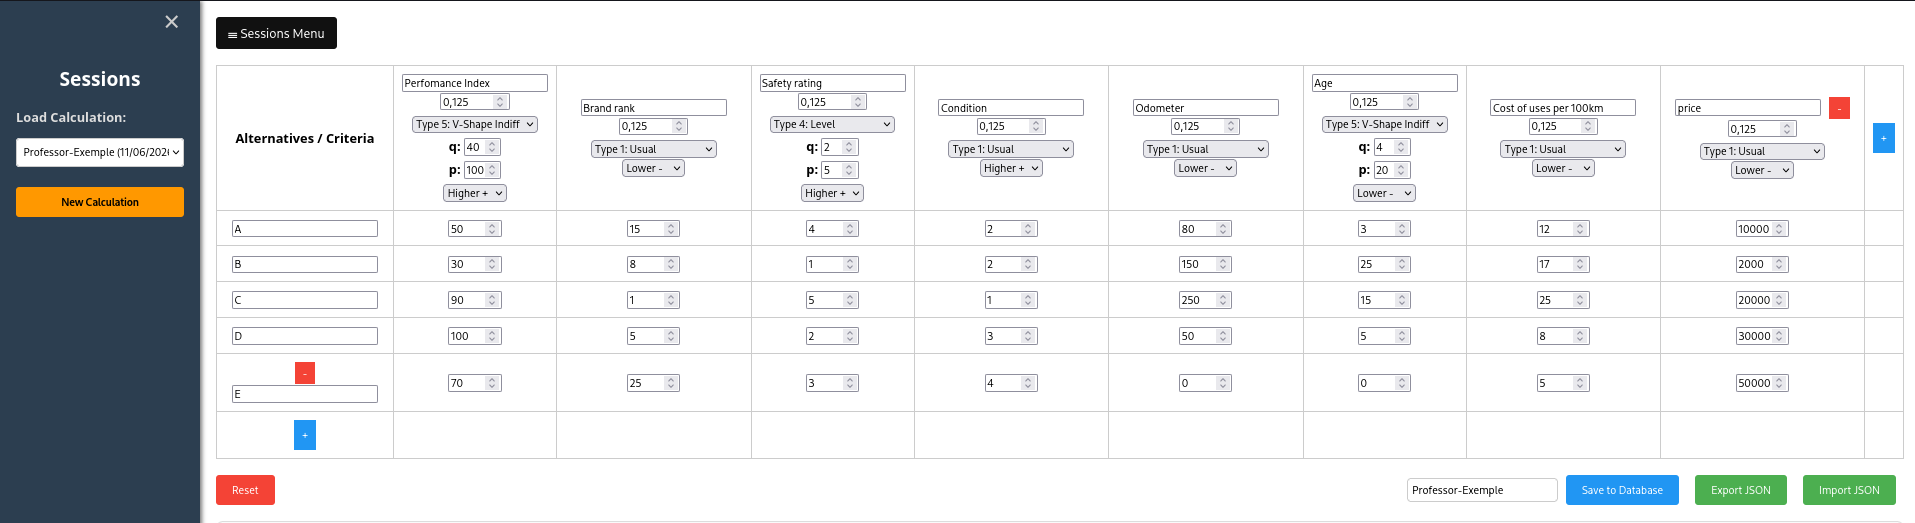
\includegraphics[width=0.95\textwidth]{./res/application_picture/Matrix_alternative_criteria.png}
  \caption{Data Entry Interface: Users can dynamically add criteria and alternatives, choosing weights and preference functions through simple dropdowns and inputs.}
  \label{fig:ui_matrix}
\end{figure}

Key functionalities include:
\begin{itemize}
    \item \textbf{Dynamic Matrix:} Real-time addition/removal of criteria and alternatives.
    \item \textbf{Real-time Calculation:} The results update automatically as soon as the criterion weights sum to 1.0.
    \item \textbf{Pairwise Analysis:} A dedicated section to compare any two alternatives criterion-by-criterion.
\end{itemize}

The interface is designed to support both roles identified in MCDA methodology: the \textbf{Decision Maker (DM)}, who inputs evaluations and interprets results, and the \textbf{Decision Analyst (DA)}, who configures the criteria, weights, and preference functions.

\section{Usage Scenario and Use Cases}
Consider a Decision Maker wishing to select a company vehicle. They open the application and create a new session named ``Vehicle Purchase 2026''. They add three alternatives (Car A, Car B, Car C) and define three criteria: Price (to minimize), Quality (to maximize), and Delivery Time (to minimize). For each criterion, they select an appropriate preference function and assign weights summing to 1.0. As they fill in the evaluation scores, the PROMETHEE II ranking updates in real time. Finally, they use the pairwise comparison tool to analyze why Car A ranks above Car C on specific criteria, and save the session for future reference.

The full set of user interactions and functionalities described in this scenario are formalized in the Use Case diagram below (see Figure \ref{fig:usecase}).

\begin{figure}[H]
  \centering
  
\includegraphics[width=0.85\textwidth]{./res/Uml/Usual_Case_Diagram.png}
  \caption{Use Case Diagram: Illustrates the primary interactions a user has with the system, such as managing the matrix and exporting results.}
  \label{fig:usecase}
\end{figure}

\section{Data Storage Overview}
The application persists four types of information to ensure full persistence: \textbf{Sessions} (the global decision problem), \textbf{Criteria} (weights and preference function parameters), \textbf{Alternatives} (names and identities), and \textbf{Evaluations} (the raw performance scores linking each alternative to each criterion). The detailed relational schema is presented in the Technical Design chapter.

%------------------------------------------------------------
\chapter{Technical Design}
%------------------------------------------------------------

\section{Implementation Choices and Technologies}
The backend is implemented using \textbf{Jakarta EE Servlets}, chosen for its robustness and my strong academic familiarity with the Java ecosystem. \textbf{Apache Tomcat 10.1} was selected for its open-source nature and widespread industry adoption as a stable Servlet container. For data persistence, \textbf{PostgreSQL} was preferred over alternatives for its strict ACID compliance and advanced support for relational data. Database connectivity is ensured via the \textbf{PostgreSQL JDBC Driver}, which enables the Jakarta EE application to communicate with the database using standard SQL queries. Finally, \textbf{Docker} was employed to ensure a fully reproducible deployment environment across different machines.

The frontend utilizes vanilla JavaScript and JavaServer Pages (JSP) to maintain high performance and avoid the overhead of heavy frameworks. To improve the user experience, the application utilizes the browser's \textbf{localStorage} to automatically cache the matrix state during editing.

\section{System Architecture and Deployment}
The application follows a classic three-tier architecture, physically distributed across multiple nodes. As detailed in the Deployment Diagram (see Figure \ref{fig:deployment}), the system consists of a client browser, an application server container, and a database container.

The two API endpoints are strictly separated by responsibility: 
\begin{itemize}
    \item \texttt{PrometheeServlet} (\texttt{/calculate}) is stateless and processes raw JSON matrix data to return computed flows.
    \item \texttt{SessionServlet} (\texttt{/api/sessions}) manages stateful CRUD operations against the PostgreSQL database.
\end{itemize}

The entire stack is orchestrated using Docker Compose, which seamlessly networks the Tomcat application container with the database container, mounting a local volume for persistent storage and initializing the schema automatically.

\begin{figure}[H]
  \centering
  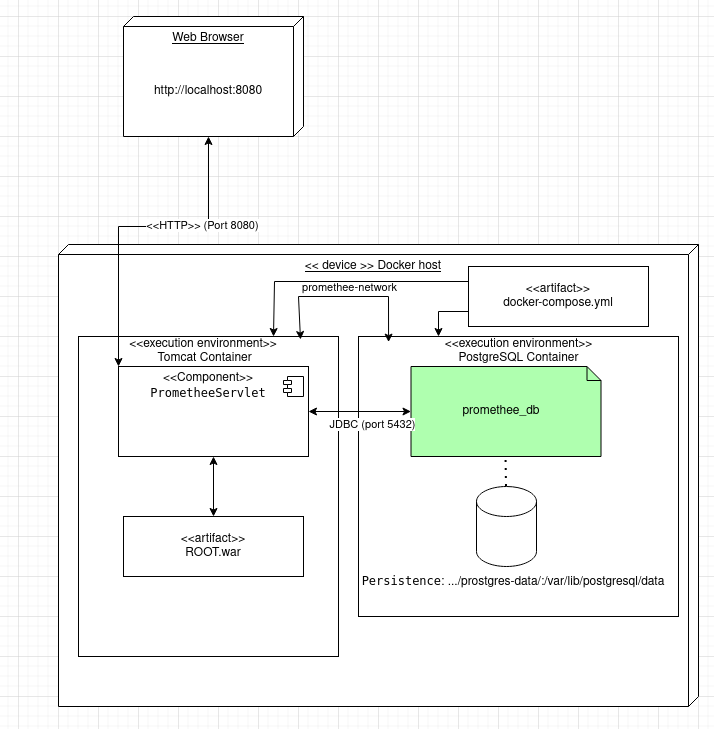
\includegraphics[width=0.85\textwidth]{./res/Uml/Diagram_Deployement.png}
  \caption{Deployment Diagram: Shows the physical distribution of the system components.}
  \label{fig:deployment}
\end{figure}

\section{Logical Data Model (MLD)}
The relational structure of the database was designed to support the PROMETHEE data model, ensuring a clear separation between session metadata, criteria parameters, and raw evaluation scores.
\begin{figure}[H]
  \centering
  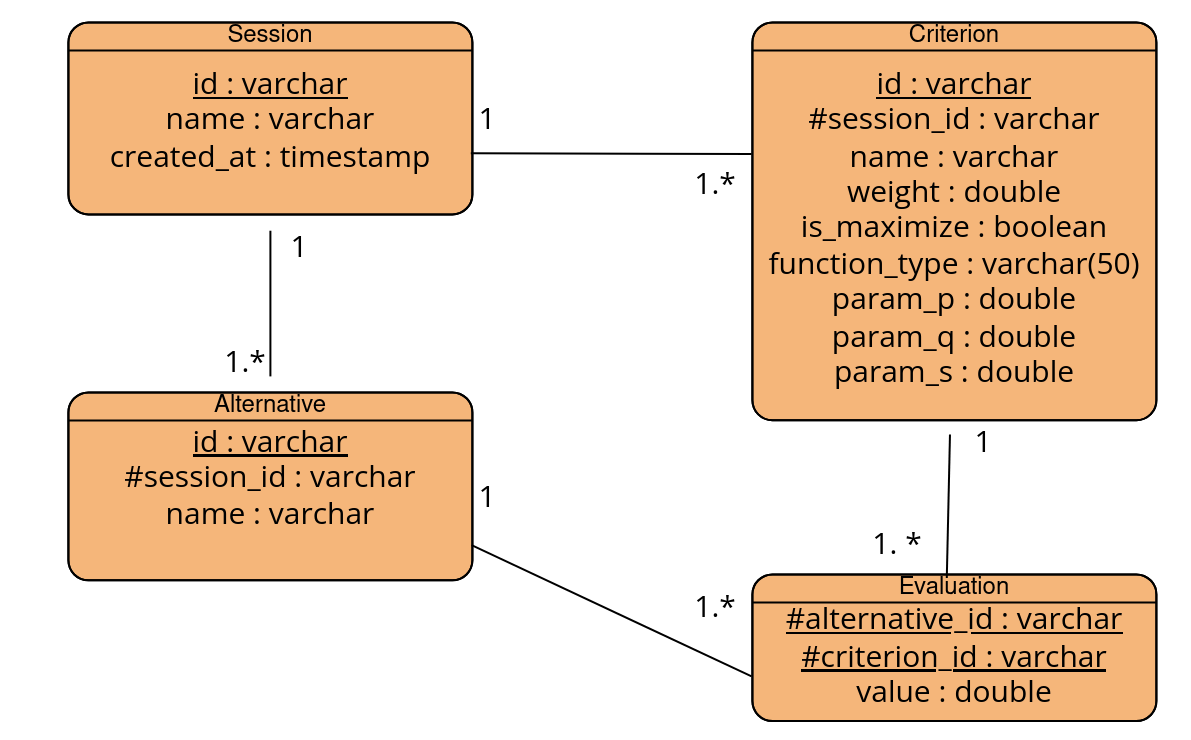
\includegraphics[width=0.85\textwidth]{./res/Uml/MLD_Database.png}
  \caption{Logical Data Model: Relational schema including primary and foreign key associations.}
  \label{fig:mld}
\end{figure}

\section{MVC and Service Layer Architecture}
To ensure maintainability and scalability, the code follows a strict Model-View-Controller (MVC) pattern, enhanced with a dedicated Service layer to decouple concerns.
\begin{itemize}
    \item \textbf{Controller:} Managed by Jakarta EE Servlets (\texttt{PrometheeServlet} and \allowbreak \texttt{SessionServlet}), which handle incoming HTTP requests and delegate logic to the service layer.
    \item \textbf{Service:} The \texttt{PrometheeService} centralizes the business logic, including JSON data parsing (utilizing the powerful \textbf{Jackson} library) and the orchestration of the mathematical calculation engine. It also implements the \textbf{DTO (Data Transfer Object)} pattern via the \texttt{CalculationResult} class to efficiently package API responses.
    \item \textbf{Model:} Classes (\texttt{Alternative}, \allowbreak \texttt{Criterion}, \allowbreak and \allowbreak \texttt{Session}) encapsulate the PROMETHEE data structures and mathematical rules.
    \item \textbf{DAO:} The \texttt{SessionDAO} handles interaction with the PostgreSQL database using standard JDBC.
\end{itemize}

\begin{figure}[H]
  \centering
  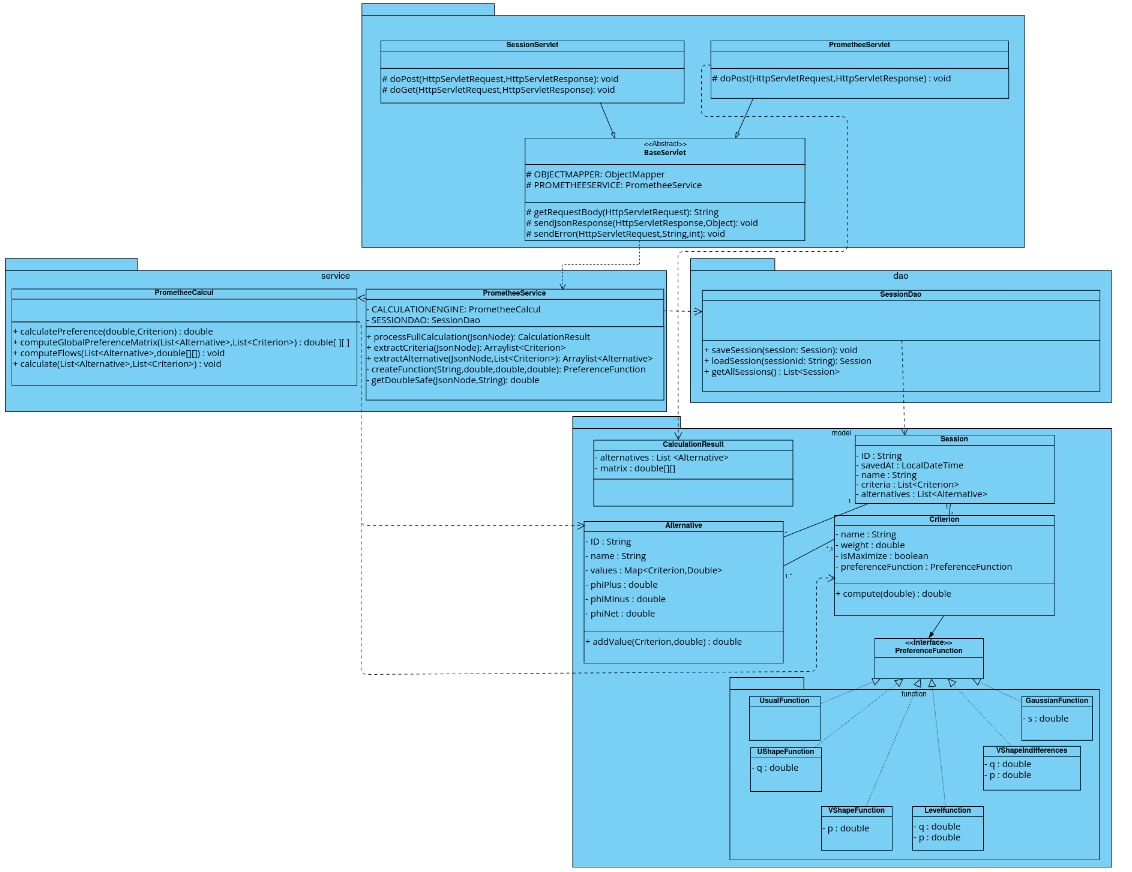
\includegraphics[width=0.85\textwidth]{./res/Uml/Diagram_class.png}
  \caption{Class Diagram: Internal object-oriented structure of the mathematical model.}
  \label{fig:classdiagram}
\end{figure}

%------------------------------------------------------------
\chapter{Discussion}
%------------------------------------------------------------

\section{Extended Experiment and Usage Example}
To validate the application, a vehicle selection scenario was implemented. Three alternatives were compared against three criteria using the parameters defined in Table \ref{tab:exp_input}.

\begin{table}[H]
\caption{Experiment Data: Input Matrix and Parameters}
\label{tab:exp_input}
\centering
\begin{tabular}{lccc}
\toprule
\textbf{Alternative} & \textbf{Price (Min, V-Shape)} & \textbf{Quality (Max, Usual)} & \textbf{Delay (Min, U-Shape)} \\
\textbf{Weight} & \textbf{w=0.5, p=10} & \textbf{w=0.3} & \textbf{w=0.2, q=5} \\
\midrule
Car A & 80 & 10 & 15 \\
Car B & 90 & 9 & 12 \\
Car C & 75 & 8 & 20 \\
\bottomrule
\end{tabular}
\end{table}

The application generated the following results (see Figure \ref{fig:ui_results}):

\begin{table}[H]
\caption{Experiment Results: Calculated Flows}
\label{tab:exp_results}
\centering
\begin{tabular}{lcccc}
\toprule
\textbf{Alternative} & \textbf{$\Phi^+$ (Power)} & \textbf{$\Phi^-$ (Weakness)} & \textbf{$\Phi$ (Net Flow)} & \textbf{Rank} \\
\midrule
Car A & 0.5500 & 0.1250 & 0.4250 & 1 \\
Car C & 0.3750 & 0.4000 & -0.0250 & 2 \\
Car B & 0.2500 & 0.6500 & -0.4000 & 3 \\
\bottomrule
\end{tabular}
\end{table}

\begin{figure}[H]
  \centering
  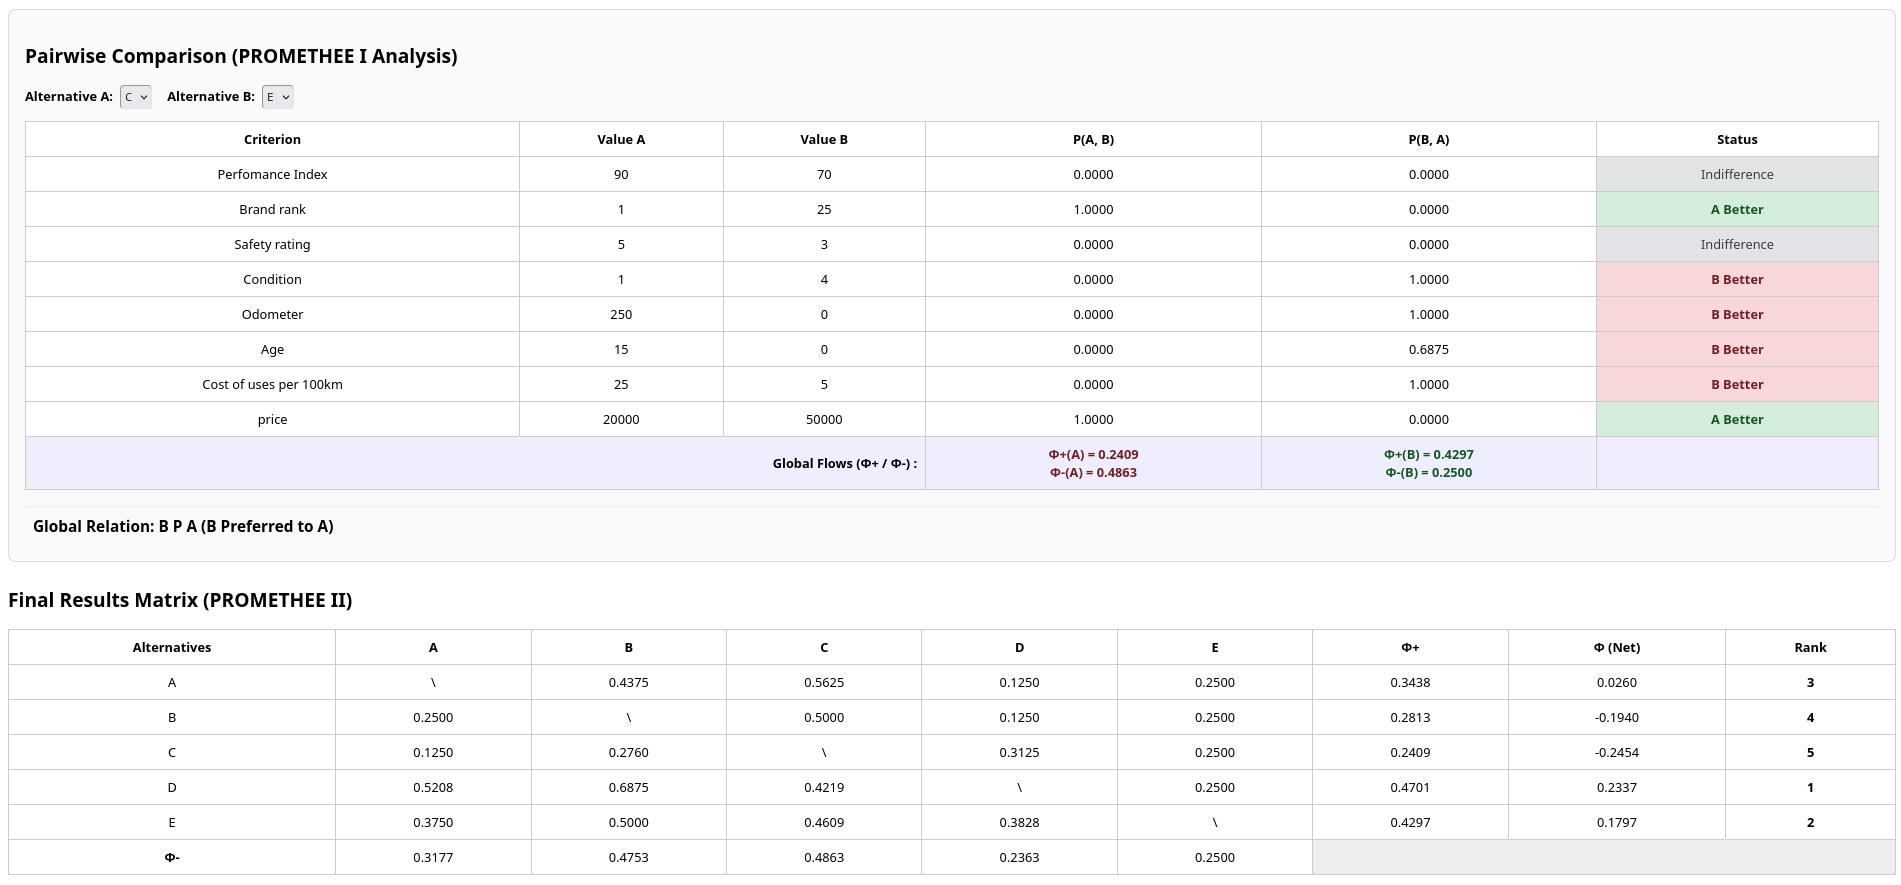
\includegraphics[width=0.95\textwidth]{./res/application_picture/Promethee_I_and_II.png}
  \caption{Results Interface: Final ranking and pairwise comparison between Car A and Car C.}
  \label{fig:ui_results}
\end{figure}

The results confirm that Car A is the best overall choice, driven primarily by its competitive price (dominant criterion with w=0.5). Car C ranks second despite its lower price because its significantly longer delivery time (20 days vs 15 for Car A) penalizes it on that criterion. Car B ranks last due to its highest price (90), which is decisively penalized by the V-Shape function with p=10.

Applying PROMETHEE I, Car A and Car C are comparable ($\Phi^+(A) > \Phi^+(C)$ and $\Phi^-(A) < \Phi^-(C)$), confirming Car A's dominance. However, Car A and Car B are also comparable, while Car B and Car C present an interesting case worth examining in the pairwise tool.

\section{Analysis: Positives and Limitations}
\textbf{Positives:} The application provides a highly responsive experience through real-time AJAX recalculations. The backend follows SOLID principles and utilizes the DTO pattern for API communication. The application also supports JSON import/export, enabling users to share and reload decision matrices across sessions.

\textbf{Limitations and Future Alternatives:} One observed limitation is that the current frontend architecture does not provide visual feedback when weights do not sum to exactly 1.0 due to floating-point precision issues (e.g., 0.1 + 0.2 + 0.7 = 0.9999... in JavaScript). A rounding mechanism was implemented as a workaround, but a more robust solution would involve server-side weight normalization.

Graphical visualizations such as the GAIA plane \cite{mareschal2013} would allow Decision Makers to better interpret conflicting criteria visually. 
Furthermore, adding multi-user authentication would transform the tool into a collaborative platform supporting multiple Decision Makers simultaneously.

%------------------------------------------------------------
\chapter{Conclusions}
%------------------------------------------------------------

\section{Synopsis of Work}
This project delivered a fully functional, containerized web application implementing the PROMETHEE I and II multi-criteria decision analysis methods. The platform provides a dynamic interface for defining complex decision problems, evaluating alternatives through six distinct preference functions, and persistently storing results in a relational PostgreSQL database. The entire stack is containerized with Docker, ensuring reproducible deployment. The backend follows SOLID principles through a strict MVC architecture with a dedicated Service layer and DAO pattern.

\section{Suggestions for Improvement}
Future iterations should focus on four axes: 
(1) modernizing the frontend architecture for better state management; 
(2) adding the GAIA plane visualization \cite{mareschal2013} for richer result interpretation; 
(3) implementing user authentication for multi-user support; and
(4) adding server-side weight normalization to eliminate floating-point precision issues.

\section{Personal Impressions}
Working with Jakarta EE Servlets deepened my understanding of the HTTP request-response lifecycle and stateless API design. Implementing the six preference functions required carefully translating mathematical specifications into robust, tested Java code --- a level of rigor I had not previously exercised. Designing the Docker Compose orchestration also introduced me to professional deployment practices. The Erasmus+ context further challenged me to communicate all technical concepts in English daily, which significantly improved my professional fluency and adaptability in an international environment.

%============================================================
%  REFERENCES
%============================================================
\cleardoublepage
\addcontentsline{toc}{chapter}{References}

\begin{thebibliography}{99}

\bibitem{brans1985}
J.P. Brans and P. Vincke, ``A Preference Ranking Organisation Method: (The PROMETHEE Method for Multiple Criteria Decision-Making),'' \textit{Management Science}, vol. 31, no. 6, pp. 647--656, 1985.

\bibitem{belton2002}
V. Belton and T. Stewart, \textit{Multiple Criteria Decision Analysis: An Integrated Approach}. Boston: Kluwer Academic Publishers, 2002.

\bibitem{mareschal2013}
B. Mareschal, ``The PROMETHEE Methods,'' in \textit{Multiple Criteria Decision Analysis: State of the Art Surveys}, J. Figueira, S. Greco, and M. Ehrgott, Eds. New York: Springer, 2013.

\bibitem{jakartaee}
Eclipse Foundation, ``Jakarta EE 10 Documentation,'' [Online]. Available: \url{https://jakarta.ee/specifications/platform/10/}.

\bibitem{jackson}
FasterXML, ``Jackson Data Processor Documentation,'' [Online]. Available: \url{https://github.com/FasterXML/jackson-docs}.

\bibitem{TomcatDoc}
Apache Software Foundation, ``Apache Tomcat 10.1 Documentation,'' [Online]. Available: \url{https://tomcat.apache.org/tomcat-10.1-doc/}.

\bibitem{PostgreSQLDoc}
PostgreSQL Global Development Group, ``PostgreSQL 16 Documentation,'' [Online]. Available: \url{https://www.postgresql.org/docs/16/index.html}.

\bibitem{DockerDoc}
Docker Inc., ``Docker Documentation,'' [Online]. Available: \url{https://docs.docker.com/}.

\end{thebibliography}

\end{document}
